\documentclass{report}

% Packages for math symbols and equations
\usepackage[T1]{fontenc}
\usepackage[utf8]{inputenc}

\usepackage[margin=1.4in]{geometry}
\usepackage{graphicx}

\usepackage{amssymb,amsthm, amsmath}
%\usepackage{mathtools}
%\numberwithin{equation}{section}

\usepackage[
natbib,
style=alphabetic,
maxbibnames=10,  
sorting=ydnt,
url=false,
doi=false,
sortcites,
defernumbers,
backref,
backend=biber
]{biblatex}
\addbibresource{bibliography.bib}

\usepackage{hyperref}

\usepackage{todonotes}
%\setuptodonotes{inline}
\usepackage{url}

\usepackage[nameinlink, capitalise, noabbrev]{cleveref}

\usepackage{xfrac}
\usepackage{nicefrac}

\usepackage{soul}

\usepackage{bbm}

\usepackage{enumitem}

%For double brackets \llbracket \rrbracket
\usepackage{stmaryrd}

\usepackage{subcaption} %For subfigures


\crefname{assumption}{Assumption}{Assumptions}

\newtheorem{theorem}{Theorem}
\newtheorem{conjecture}{Conjecture}
\newtheorem*{theorem*}{Theorem}
\newtheorem*{conjecture*}{Conjecture}
\newtheorem{claim}{Claim}

\newtheorem{proposition}{Proposition}[section]
\newtheorem{notation}{Notation}[section]
\newtheorem{lemma}{Lemma}[section]
\newtheorem{corollary}{Corollary}[section]
\theoremstyle{remark}
\newtheorem{remark}{Remark}[section]


\theoremstyle{definition}
\newtheorem{example}{Example}[section]
\newtheorem{counterexample}{Counterexample}[section]
\newtheorem{definition}{Definition}[section]
\newtheorem{assumption}{Assumption}
\newtheorem{question}{Question}
\newtheorem{exercise}{Exercise}
\newtheorem{fact}{Fun Fact}
%\numberwithin{equation}{section}

%\renewcommand{\baselinestretch}{2}

%\newcounter{hypcounter}

\newcommand{\N}{\mathbb{N}}
\newcommand{\Z}{\mathbb{Z}}
\newcommand{\R}{\mathbb{R}}
%\DeclareMathOperator{\dom}{dom}
\newcommand{\closure}[1]{\overline{#1}}
\newcommand{\norm}[1]{\left\Vert #1 \right\Vert}
\newcommand{\seminorm}[1]{\left[ #1 \right]}
\newcommand{\abs}[1]{\left\vert #1 \right\vert}
%\DeclareMathOperator{\divtmp}{div}
\renewcommand{\div}{\divtmp}
% \DeclareMathOperator{\argmin}{arg\,min}
% \DeclareMathOperator{\argmax}{arg\,max}
% \DeclareMathOperator{\esssup}{ess\,sup}
% \DeclareMathOperator{\essinf}{ess\,inf}
\renewcommand{\st}{\,:\,}
% \DeclareMathOperator{\supp}{supp}
\newcommand{\dx}{\,\mathrm{d}x}
\renewcommand{\d}{\,\mathrm{d}}
\newcommand{\dH}{\,\mathrm{d}\mathcal{H}^{n-1}(x)}
% \DeclareMathOperator{\sign}{sign}
\newcommand{\eps}{\varepsilon}
% \DeclareMathOperator{\dist}{dist}
% \DeclareMathOperator{\Lip}{Lip}
\newcommand{\KR}{\mathrm{KR}}
\newcommand{\C}{\mathrm{C}}
\renewcommand{\L}{\mathrm{L}}
\newcommand{\W}{\mathrm{W}}
\newcommand{\M}{\mathcal M}
\newcommand{\grad}{\nabla}
\newcommand{\hess}{\mathrm{D}^2}
\newcommand{\defeq}{:=}
% \DeclareMathOperator{\diam}{diam}
\newcommand{\Set}[1]{\left\lbrace#1\right\rbrace}
\newcommand{\scale}{\eps}
\newcommand{\res}{\delta}


\newcommand{\wto}{\rightharpoonup}
\newcommand{\wsto}{\overset{\ast}{\rightharpoonup}}
\newcommand{\strictto}{\overset{\mathrm{str}}{\rightharpoonup}}

\newcommand{\rev}{\color{magenta}}
\renewcommand{\rev}{}
\newcommand{\red}{\color{red}}
\newcommand{\blue}{\color{blue}}
\newcommand{\nc}{\normalcolor}


% Lie math operators
\DeclareMathOperator{\toledo}{T}
\DeclareMathOperator{\isom}{Isom}
\DeclareMathOperator{\bus}{b}
\DeclareMathOperator{\ii}{i}
\DeclareMathOperator{\spa}{span}
\DeclareMathOperator{\class}{C}
\DeclareMathOperator{\diam}{diam}
\DeclareMathOperator{\diag}{diag}
\DeclareMathOperator{\U}{{\mathrm{U}}}
\DeclareMathOperator{\OO}{{\mathrm{O}}}
\DeclareMathOperator{\SL}{{\mathrm{SL}}}
\DeclareMathOperator{\SU}{{\mathrm{SU}}}
\DeclareMathOperator{\Sp}{{\mathrm{Sp}}}
\DeclareMathOperator{\su}{{\mathfrak{su}}}
\DeclareMathOperator{\PSL}{{\mathrm{PSL}}}
\DeclareMathOperator{\GL}{{\mathrm{GL}}}
\DeclareMathOperator{\gl}{{\mathfrak{gl}}}
\DeclareMathOperator{\SO}{{\mathrm{SO}}}
\DeclareMathOperator{\sso}{{\mathfrak{so}}}
\DeclareMathOperator{\PGL}{{\mathrm{PGL}}}
\DeclareMathOperator{\PO}{{\mathrm{PO}}}
\DeclareMathOperator{\PSO}{{\mathrm{PSO}}}
\DeclareMathOperator{\id}{id}
\DeclareMathOperator{\inte}{int}
\DeclareMathOperator{\LC}{LC{}}
\DeclareMathOperator{\F}{Frenet{}}
\DeclareMathOperator{\lie}{Lie}
\DeclareMathOperator{\Ker}{Ker}
\DeclareMathOperator{\ad}{ad}
\DeclareMathOperator{\Hff}{dim_{Hf{}f}}
\DeclareMathOperator{\vol}{Vol}
\DeclareMathOperator{\rk}{rank}
%\DeclareMathOperator{\jac}{jac}
\DeclareMathOperator{\gap}{{\sf{gap}}}
\DeclareMathOperator{\ann}{Ann}
\DeclareMathOperator{\tr}{tr}
\DeclareMathOperator{\Ad}{Ad}
\DeclareMathOperator{\Sym}{Sym}
\DeclareMathOperator{\Isom}{Isom}
\DeclareMathOperator{\Stab}{Stab}
\DeclareMathOperator{\II}{I\!I} % second fundamental form
\DeclareMathOperator{\sgn}{sgn} % second fundamental form


%AntideSitter spaces and Teichmuller theory
\DeclareMathOperator{\fut}{\mathrm{I}^+}
\DeclareMathOperator{\futc}{\mathrm{J}^+}
\DeclareMathOperator{\past}{\mathrm{I}^-}
\DeclareMathOperator{\pastc}{\mathrm{J}^-}
\DeclareMathOperator{\dom}{\mathcal D}
\DeclareMathOperator{\CH}{\mathrm{CH}}
%:= sign
\newcommand{\equaldef}{\overset{\mathrm{def}}{=}}

\newcommand{\restr}{\mathbin{\vrule height 1.6ex depth 0pt width
0.13ex\vrule height 0.13ex depth 0pt width 1.3ex}}

\usepackage{tikz-cd}


% Title page information
\title{Notes}
\author{Giorgos}
\date{\today}

\begin{document}

\maketitle

\tableofcontents

\chapter{Lorentzian spaces}
Here we recall some basic facts on Lorentzian spaces.
We will introduce Lorentzian manifolds of constant sectional curvature and we will see that, as in the Riemannian case, two Lorentzian manifolds of constant sectional curvature $K$ are locally isometric.
Generally, we will focus on those with maximal isometry group, as they provide models of manifolds of constant sectional curvature: if $M$ is a Lorentzian manifold with constant sectional curvature $K$ and maximal isometry group, then any Lorentzian manifold with constant sectional curvature $K$ carries a natural $(\mathrm{Isom}(M), M)$-atlas made of local isometries. Simply connected space forms have maximal isometry group, but in general there are manifolds with maximal isometry group which are not simply connected.
In particular, we will focus on the case $K=-1$ and in that case it will be convenient to use  models which are not simply connected.

\section{Basic definitions}
\begin{definition}
    \begin{enumerate}[label=(\roman*)]
        \item A \emph{Lorentzian metric} on a manifold of dimension $n+1$  is a non-degenerate symmetric 2-tensor $g$ of signature $(n,1)$. 
        \item A \emph{Lorentzian manifold} is a connected manifold $M$ equipped with a Lorentzian metric $g$.
        \item In a Lorentzian manifold $M$ we say that a non-zero vector $v\in TM$ is \emph{spacelike, lightlike, timelike} if $g(v,v)$ is respectively positive, zero or negative. More generally, we say that a linear subspace $V\subset T_x M$ is \emph{spacelike, lightlike, timelike} if the restriction of $g_x$ to $V$ is positive definite, degenerate or indefinite.
        \item A differentiable curve is \emph{spacelike, lightlike, timelike} if its tangent vector is spacelike (resp. lightlike, timelike) at every point. It is \emph{causal} if the tangent vector is either timelike or lightlike.
        \item The set of lightlike vectors of $T_x M$ is also known as the \emph{light cone} at $x$.
    \end{enumerate}
\end{definition}

Assuming $\dim M \geq 3$, the light cone disconnects $T_x M$ into three regions: two convex open cones formed by timelike vectors, one opposite to the other, and the region of spacelike vectors.
\begin{definition}
    Let $M$ be a Lorentzian manifold.
    \begin{enumerate}[label=(\roman*)]
        \item A continuous choice (in the sense of a continuous timelike vector field) of one of the two cones of time-like vectors for each point $x\in M$ is called a \emph{time orientation} of $M$.
        \item If a time-orientation of $M$ exists, then $M$ is said to be \emph{time-orientable}.
        Timelike vectors in the same component as the time-orientation are said \emph{future-directed}, while the rest are said \emph{past-directed}.
        \item Given a point $x$ in a time-oriented Lorentzian manifold $M$, the \emph{future} of $x$ is the set $\fut{(x)}$ of points which are connected to $x$ by a future-directed causal curve. The \emph{past} of $x$, denoted $\past{(x)}$, is defined similarly, for past-directed causal curves.
    \end{enumerate}
\end{definition}

An \emph{orthonormal basis} of $T_xM$ is a basis $v_1,\ldots v_{n+1}$ such that $|g(v_i, v_j)|=\delta_{ij}$, with $v_1,\ldots v_n$ spacelike, and  $v_{n+1}$ timelike.
As in the Riemannian setting, on a Lorentzian manifold $M$ there is a unique linear connection $\nabla$ which is symmetric and compatible with the Lorentzian metric $g$.
We refer to it as the \emph{Levi-Civita connection} of $M$. The Levi-Civita connection determines the Riemann curvature tensor  defined by
$$R(u,v)w=\nabla_u \nabla_v w-\nabla_v \nabla_u w-\nabla_{[u,v]}w~.$$
We then say that a Lorentzian manifold $M$ has constant sectional curvature $K$ if
\begin{equation}\label{eq:constcurv}
     g(R(u,v)v,u)=K \left(g(u,u)g(v,v)-g(u,v)^2\right)
\end{equation}
for every pair of vectors $u,v\in T_xM$ and every $x\in M$.
This definition is strictly analogous to the definition given in the Riemannian realm. However in this setting the sectional curvature can be defined only for planes in 
$T_x M$ where $g$ is non-degenerate.
\begin{example}
The Minkowski space $\R^{n,1}$ the Levi-Civita connection given by the Euclidean connection:
\[
\nabla_X Y = (X Y^i)\partial_i,
\]
so the Riemann curvature tensor is zero, and the same is true for the sectional curvature.
\end{example}

Finally, we say that $M$ is \emph{geodesically complete} if every geodesic is defined for all times, or in other words, the exponential map is defined everywhere.

\section{Maximal isometry groups and geodesic completeness}
Constant curvature of manifolds allows us to extend isometries of tangent spaces to isometries of the whole manifold.
As a result, two Lorentzian manifolds $M$ and $N$ of constant curvature $K$ are locally isometric, a fact which is well-known in the Riemannian setting. 
More precisely, the following holds:
\begin{lemma} \label{lem:extension}
Let $M$ and $N$ be Lorentzian manifolds of constant curvature $K$. 
\begin{enumerate}
    \item Then every linear isometry $L:T_xM\to T_yN$ extends to an isometry $f:U\to V$, where $U$ and $V$ are neighbourhoods of $x$ and $y$ respectively, and two extensions $f:U\to V$ and $f:U'\to V'$ of $L$ coincide on $U\cap U'$.
    \item If $M$ is simply connected and $N$ is geodesically complete, then any isometry $L: T_x M \to T_y N$ extends to a unique local isometry $f:M\to N$.
    \item If $M$ and $N$ are both simply connected and geodesically complete, then any isometry $L: T_xM\to T_yN$ extends to a unique global isometry $f:M\to N$.
\end{enumerate}
\end{lemma}
\begin{proof}
    For the last statement, recall that a local isometry from a simply connected manifold to a uniquely geodesic manifold is a global isometry.
\end{proof}
Exactly as in the Riemannian case the proof is a simple consequence of the classical Cartan--Ambrose--Hicks Theorem.
Note that this implies in particular that there is a unique simply connected geodesically complete Lorentzian manifold of constant curvature $K$ up to isometries.
For instance for $K=0$ a model is the Minkowski space $\R^{n,1}$.

Another consequence of Lemma \ref{lem:extension} is that, fixing a point $x_0\in M$, the set of isometries of $M$, which we will denote by $\mathrm{Isom}(M)$, can be realized as a subset of $\mathrm{ISO}(T_{x_0}M, TM)$, namely the fiber bundle over $M$ whose fiber over $x\in M$ is the space of linear isometries of $T_{x_0}M$ into $T_x M$.

It can be proved that $\mathrm{Isom}(M)$ has the structure of a Lie group with respect to composition so that the inclusion
$\mathrm{Isom}(M)\hookrightarrow\mathrm{ISO}(T_{x_0}M, TM)$ is a differentiable proper embedding.
It follows that  the maximal dimension of $\mathrm{Isom}(M)$ is
 $\dim \OO(n,1)+n+1=(n+1)(n+2)/2$. 
 
\begin{definition}
A Lorentzian manifold $M$ has \emph{maximal isometry group} if the action of $\mathrm{Isom}(M)$ is transitive and, 
for every point $x\in M$, every linear isometry $L:T_xM\to T_xM$ extends to an isometry of $M$.
\end{definition}
Equivalently $M$ has maximal isometry group if the above inclusion of $\mathrm{Isom}(M)$ into the bundle $\mathrm{ISO}(T_{x_0}M, TM)$ is a bijection.
Hence, if $M$ has maximal  isometry group, then the dimension of the isometry group is maximal.

From \cref{lem:extension}, every simply connected Lorentzian manifold $M$ has maximal isometry group if it has constant sectional curvature and is geodesically complete. The converse holds even without the simply connectedness assumption:
\begin{lemma} \label{lemma:max isom group implies constant curvature}
\begin{enumerate}[label=(\roman*)]
    Let $M$ be a Lorentzian manifold.
    \item If $M$ has a maximal isometry group then $M$ has  constant sectional curvature and is geodesically complete.
    \item If $M$ is simply connected, then $M$ has maximal isometry group if and only if $M$ has constant sectional curvature and is geodesically complete.
\end{enumerate}
\end{lemma}

\chapter{Linear algebra}
\section{Proximal elements in $\GL(n,\R)$}
Here we will talk about basic definitions and dynamics of proximal elements in $\GL(n,\R)$ and its subgroups.
\begin{definition}
    We say that $g \in \PGL(d, \mathbb R)$ is \emph{proximal} (in $\mathbb P(\mathbb R^d)$) if it admits an attractive fixed point in $\mathbb P(\mathbb R^d)$, i.e. there exists a line $x_g^+ \in \mathbb P(\mathbb R^d)$ and a compact neighborhood $b^+ \subseteq \mathbb P(\mathbb R^d)$ of $x+g^+$ such that $g^n x \to x $ as $n \to \infty$ uniformly for $x \in b^+$.
    We say that $g$ is biproximal if both $g$ and $g^{-1}$ are proximal.
\end{definition}

To better understand the dynamics of proximal elements, we will recall the Jordan decomposition of a matrix.
Let $A \in \GL(d,\mathbb R)$.
Then $A$ admits a Jordan canonical form $A = B J B^{-1}$, where $B \in \GL(d, \mathbb R)$ and $J$ is a block diagonal matrix with Jordan blocks $J_1, \ldots, J_k$:
\[
J = \begin{pmatrix}
    J_1 & & \\
    & \ddots & \\
    & & J_m
\end{pmatrix},
\]
where each $J_i$ is either a single real entry $j_i$, or a (real) Jordan block of the form
\[
J_i = \begin{pmatrix}
    C_i & 1 & & \\
    & C_i & \ddots & \\
    & & \ddots & 1 \\
    & & & C_i
\end{pmatrix},
\]
with $C_i$ being a $2 \times 2$ matrix of the form
\[
C_i = \begin{pmatrix}
    a_i & -b_i \\
    b_i & a_i
\end{pmatrix},
\]
and $b_i \neq 0$.
In the latter case, we let $j_i$ be one of the complex eigenvalues $j_i = \sqrt{\det C_i} e^{i \arccos(a_i)}$ of $C_i$.
\begin{remark}
    Each $C_i$ is merely a similitude (in case $C_i$ is not a single entry) by $|j_i| = \sqrt{\det C_i}$ of a rotation by $\arccos a_i$, so $J_i$ rotates and multiplies the plane corresponding to its first two collumns.
\end{remark}
We call each $j_i$ a \emph{generalised eigenvalue} of $A$ and the subspace $E_i$ preserved by each $J_i$ the \emph{generalised eigenspace} of $j_i$.
By changing $B$ we may assume that $|j_1| \geq \ldots \geq |j_m|$.

We are now ready to describe the dynamics of a Jordan block, which is the same as the dynamics of $A$ in the respective generalised eigenspace.
\begin{lemma}[Dynamics of a Jordan block]
    Let $J_i$ be a Jordan block, and let $j_i, E_i$ be its generalised eigenvalue and eigenspace respectively.
    We denote with $e_1, \cdots, e_k$ part of the standard basis that spans $E_i$.
    \begin{enumerate}[label=(\roman*)]
        \item There exists vectors $v \in E_i$ such that
        \[
        |J_i^n v| = |j_i|^n |v|.
        \]
        When $C_i$ is a real entry, this holds for $v \in \mathbb Rv_1$, while when $C_i$ is a $2 \times 2$ matrix, this holds for $v \in \mathbb R e_1 \oplus \mathbb R e_2$.
        \item If $J_i$ is upper-triangular but not a single entry, then $E_i$ contains an actual eigenvector (namely $e_1$) such that for $v \in E_i$ we have $J_i^n \mathbb Rv \to \mathbb Re_1$.
    \end{enumerate}
    \begin{proof}
        While we will not give a concrete proof of this fact, we can consider examples.
        \begin{enumerate}[label=(\roman*)]
            \item This follows by the fact that for $v$ in the respective subspaces, $J_i$ is a similitude by $j_i$ and perhaps a rotation.
            \item 
            Suppose $J$ is $2\times 2$, so
            \[
            J_i = \begin{pmatrix}
                a_i & 1 \\
                0 & a_i
            \end{pmatrix}.
            \]
            Then for $w = w_1 e_1 + w_2 e_2 \in E_i$ we have
            \[
            J_i \mathbb R w = \mathbb R(w + a_i w_2 e_1).
            \]
            Then it is clear to see that $J_i^n \mathbb R w \to \mathbb R e_1 $ and that $J_i$ moves lines clockwise when $a_1 > 0 $ and counterclockwise when $a_1 < 0$.
            (see \cref{fig:jordan_dynamics}).
            \begin{figure}[ht]
                \centering
                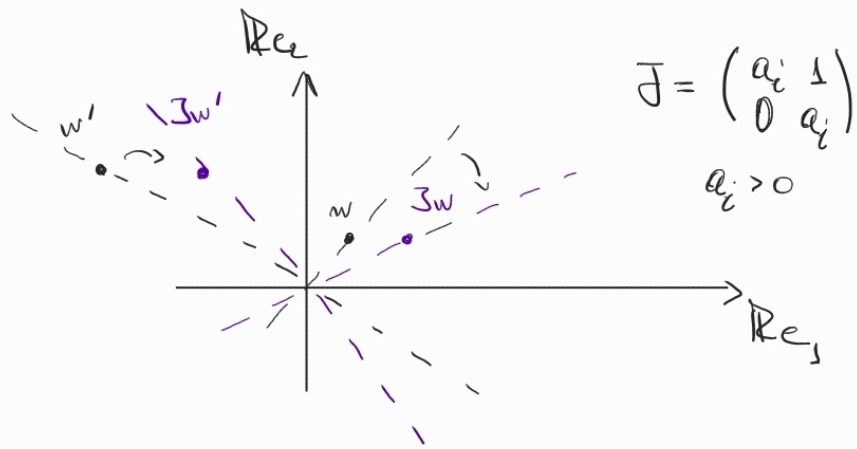
\includegraphics[width=0.7\textwidth]{jordan_dynamics.jpg}
                \caption{Dynamics of a Jordan block}
                \label{fig:jordan_dynamics}
            \end{figure}
        \end{enumerate}
    \end{proof}
    \begin{remark}
        Even when a Jordan block upper triangular and is not a single entry, the eigenline may not be an attracting fixed point since the convergence is not uniform.
        Take for example 
        \[
        J = \begin{pmatrix} 1 & 1 \\ 0 & 1 \end{pmatrix} \text{ and } v_n = (n, -1).
        \]
        Then $J^n v_n = (0, -1)$, even though $v_n \to e_1, J^n \mathbb R v_{n_0} \to \mathbb R e_1$ as $n \to \infty$ .
    \end{remark}
\end{lemma}

We now consider the Jordan matrix (see \cref{fig:jordan_matrix_dynamics}):
\begin{proposition}[Dynamics of a Jordan matrix]
    Let $J$ be a Jordan matrix with Jordan blocks $J_1, \cdots J_m$.
    Then $J$ is proximal if and only if $|j_1| > |j_2|$ and $ J_1$ is a real entry.
    In that case, for any $x \in \spa \{e_2, \cdots, e_d \}^c$ we have
    \[
    J^n x \to \mathbb R e_1,
    \]
    and the convergence is uniform in compact neighborhoods of $\spa \{e_2, \cdots, e_d \}^c$.
    Similarly, $J$ is biproximal if and only if $|j_1| > |j_2|, |j_{m-1}| > |j_m|$ and $J_1, J_m$ are real entries.
    In that case, for any $x \in \spa \{e_1, \cdots, e_{d-1} \}^c$ we have
    \[
    J^{-n} x \to \mathbb R e_d,
    \]
    and the convergence is uniform in compact neighborhoods of $\spa \{e_1, \cdots, e_{d-1} \}^c$.
\end{proposition}
\begin{proof}
    Note that if $|j_1| > |j_2|$ and $J_1$ is a real entry, then for $w \not \in \spa{ e_2, \cdots, e_d}$, we can write $w = w_1 + \cdots + w_m$ with each $w_i \in E_i$.
    Then 
    \[
    J^n \mathbb R w = \mathbb R (J_1^n w_1 + \cdots + J_m^n w_m) = 
    \mathbb R (w_1 + \frac{J_2^n}{j_1^n} w_2 + \cdots + \frac{J_m^n}{j_1^n} w_m) \to \mathbb R e_1,
    \]
    where the last convergence holds since each of the eigenvalues $j_i$ are less than $j_1$.

    If on the other hand $J$ is proximal, we have seen that in the remark above, that $J_1$ needs to be a single entry, otherwise the convergence is not uniform.
    On the other hand, if $|j_1| = |j_2|$, then $J$ will rotate the plane spanned by $e_2, e_3$, like for instance when
    \[
    J = \begin{pmatrix}
        1 & 0 & 0 \\
        0 & \cos \theta & - \sin \theta \\
        0 & \sin \theta & \cos \theta
    \end{pmatrix}, v = (1, x, y), J^n v = \begin{pmatrix}
        1\\
        \begin{pmatrix}
            \cos n \theta & - \sin n \theta \\
            \sin n \theta & \cos n \theta
        \end{pmatrix}
        \begin{pmatrix}
            x \\ y
        \end{pmatrix}
    \end{pmatrix}
    \]
\end{proof}
\begin{figure}[ht]
    \centering
    \begin{subfigure}[b]{0.45\textwidth}
        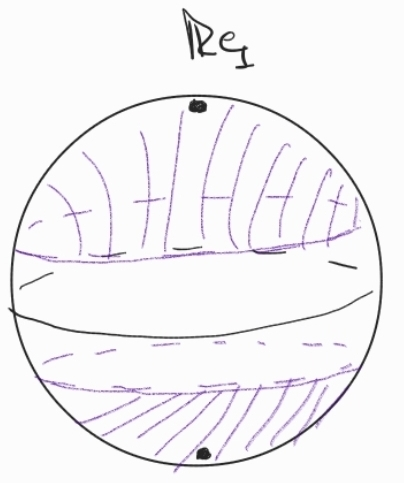
\includegraphics[width=\textwidth]{jordan_dynamics3}
        \caption{In the double cover $S^2$ convergence is uniform when uniformly away from the equator.}
        \label{fig:jordan_dynamics_sphere}
    \end{subfigure}
    \hfill
    \begin{subfigure}[b]{0.45\textwidth}
        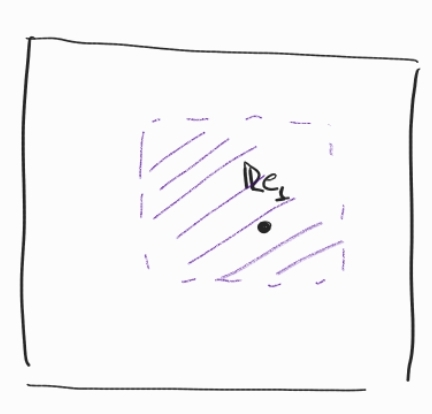
\includegraphics[width=\textwidth]{jordan_dynamics2}
        \caption{In the affine chart $\mathbb R^2 \simeq \{ [1, x, y] \}$, convergence is uniform when uniformly away from the circle at infinity.}
        \label{fig:jordan_dynamics_affine_chart}
    \end{subfigure}
    \caption{Dynamics of Jordan matrix on $\mathbb P(\mathbb R^3)$}
    \label{fig:jordan_matrix_dynamics}
\end{figure}
Noting that being proximal is invariant under conjugation, we can now describe the dynamics of a proximal element in $\GL(d, \mathbb R)$:
\begin{corollary}
    Let $g \in \PGL(d, \mathbb R)$ and denote with $g$ any of its representatives.
    Then the following are equivalent:
    \begin{enumerate}[label=(\roman*)]
        \item $g$ is proximal if and only if $g$ has a Jordan decomposition $g = B J B^{-1}$ with $J$ being proximal.
        \item Denoting with $\lambda_1(g), \cdots \lambda_d(g)$ the (possibly complex) eigenvalues of $g$ in decreasing order of their modulus, $g$ is proximal if and only if $|\lambda_1(g)| > |\lambda_2(g)|$.
    \end{enumerate}
    and similarly for biproximal elements:
    \begin{enumerate}[label=(\roman*)]
        \item $g$ is biproximal if and only if $g$ has a Jordan decomposition $g = B J B^{-1}$ with $J$ being biproximal.
        \item Denoting with $\lambda_1(g), \cdots \lambda_d(g)$ the (possibly complex) eigenvalues of $g$ in decreasing order of their modulus, $g$ is proximal if and only if $|\lambda_1(g)| > |\lambda_2(g)|$ and $|\lambda_{d-1}(g)| > |\lambda_d(g)|$.
    \end{enumerate}
    If this is the case, the attracting fixed point of $g$ is the line spanned by the eigenvector $Be_1$ and the convergence is uniform in compact neighborhoods of $\spa \{Be_2, \cdots, Be_d \}^c$.
\end{corollary}

Considering the case of $\PO(p, q)$ for $p, q \geq 0$, we have that every proximal element is biproximal:
\begin{proposition}
    In $\PO(p, q)$, proximality and biproximality are equivalent.
\end{proposition}
\begin{proof}
    Let $g \in \PO(p, q)$ be proximal.
    Then the eigenvalues of $g$ are stable under taking inverse: $\lambda(g) = \lambda(g^{-1})$.
    Indeed, $g \in \OO(p,q)$ implies that $g^t I_{p,q} g = I_{p,q}$, so for an eigenvector $v$ of $g$ with eigenvalue $\lambda$, we multiply $gv = \lambda v$ by $I_{p,q}$ to obtain that 
    \[
    \lambda I_{p,q} v =I_{p,q} g v = (g^t)^{-1} I_{p,q} v,
    \]
    so $\sigma(g) \subseteq \sigma((g^t)^{-1}) = \sigma(g^{-1})$.
\end{proof}
\printbibliography
\end{document}